\chapter{Durchführung}

\section{$\alpha_p$-Studie (VR)}
Zur Maximierung der Zugfestigkeit der Legierung Ti-6242 wurde zuerst der Einfluss des $\alpha_p$-Phasenanteils auf die Härte untersucht. Laut Lutjering und Williams sollte bei der Legierung IMI 834, eine vergleichbare Legierung zu Ti-6242, eine maximale Zugfestigkeit bei einem $\alpha_p$-Anteil von 10--20\% festgestellt werden \cite{Lutjering.2007}. Um eine größtmögliche Härtesteigerung gegenüber der as-received-Probe (AR) zu erzielen, wurden vier Proben bei unterschiedlichen Temperaturen $1h$ unterhalb der $\beta$-Transus-Temperatur geglüht und anschließend luftgekühlt (AC: air cooled) (\ref{tab:alphap}). Dabei stellt sich ein bimodales Gefüge ein. Die vier Proben wurden inklusive einer AR-Probe metallografisch präpariert und ausgewertet.

\begin{table}
	\centering
	\begin{tabular}{|c|c|c|c|}
	\hline 
	Probenbezeichnung & Temperatur [$^\circ C$] & Zeit [$h$] & Abkühlmethode \\ 
	\hline 
	BM990 & 990 & 1 & AC\\ 
	\hline 
	
	BM975 & 975 & 1 & AC\\ 
	\hline 
	BM960 & 960 & 1 & AC\\ 
	\hline 
	\end{tabular} 
	\caption{Wärmebehandlung der $\alpha_p$-Studie}
	\label{tab:alphap}
\end{table}

\pagebreak

\section{Martensit-Bildung (ZB)}

Um Martensit zu bilden wird Ti-64 nach der ersten Wärmebehandlung laut Abbildung \ref{STDA} für $1 min$  bei $930^\circ C$ geglüht und dann auf Raumtemperatur wassergekühlt. Unter dem Einfluss der Diffusion sollen $\beta$-Lamellen im transformierten $\beta$ wachsen. Die kurze Erwärmungszeit soll dafür sorgen, dass sich die neu gebildeten $\beta$-Gebiete nicht mit $\beta$-Stabilisatoren, in diesem Fall Vanadium, anreichern und dadurch stabilisiert werden. Dieser Prozess läuft im Nanometerbereich ab. Durch das schnelle Abschrecken auf Raumtemperatur wandeln sich die vergrößerten $\beta$-Bereiche diffusionslos und lokal in Martensit um.

\begin{figure}[H]
	\centering
	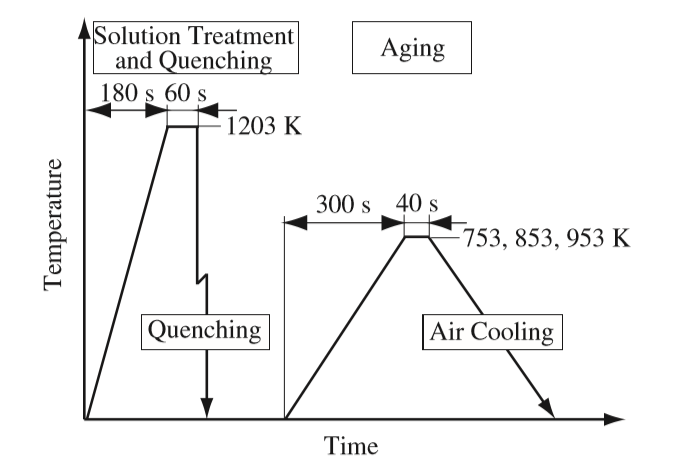
\includegraphics[width=0.9\textwidth]{Bilder/ts-stda}
	\caption{Vorgehensweise nach dem Duplex-Anneal bei STDA für Ti-64 \cite{Morita.2005}}
	\label{STDA}
\end{figure}

Da die $T_{\beta}$ von Ti-64 niedriger ist als die von Ti-6242, liegt auch ihre Gleichgewichtstemperatur unterhalb der von Ti-6242. Außerdem hat Vanadium im Vergleich zu Molybdän eine größere Diffusionsrate in Titan, was die kürzeren Anlasszeiten bei Ti-64 erklärt \cite{Zwicker.2014}. Deswegen wurden in diesem Schritt die Ti-6242-Proben nach dem Duplex-Glühen für 8 und 16 $min$ jeweils bei 930$^\circ$C und $950^\circ C$ wärmebehandelt.

Eine bekannte Wärmebehandlung von $\alpha$+$\beta$-Titanlegierungen ist die  \textit{Solution treatment and quenching}, wobei die Titanlegierung direkt von einer Temperatur $T_{1}$ unterhalb $T_{\beta}$ nach 0,5--1 h abgeschreckt wird. Wie bei der oben beschriebenen Wärmebehandlung stellt sich bei $T_{1}$ ein zweiphasiges Gefüge mit $\alpha_p$ und $\beta$ ein. Die $\beta$-Phase wandelt sich  dann beim Abschrecken martensitisch um und wird $\alpha^\prime$ genannt \cite{Morita.2005}. Zum Vergleich zu der studierten Wärmebehandlung werden AR-Proben bei $983^\circ C$ für 1h erwärmt und wassergekühlt.

\section{Martensit-Zerfall (TJ)}
Um die Härte der Legierung zu steigern, lässt man das Martensit im transformierten $\beta$ partiell zerfallen. Das passiert, indem sich das Martensit in $\alpha$ + $\beta$ umwandelt. Dadurch, dass Martensit Bildung im Nanometer Bereich stattfindet, erfolgt die Bildung mehrere kleine Lamellen. Im Material herrschen extrem kleine Diffusionsvorgänge. Der Martensit ist darin als lokales Gefüge zu finden. Hier für wird für die Wärmebehandlung weniger Zeit benötigt.

Die Probe $983\circ C$ /1h/AC + $950\circ C$ /16min/WQ ist für die nächsten Vorgänge ausgewählt worden. Dazu wurde eine kleine Studie erstellt. Untersucht wurde, ob bei zwei verschiedene Temperaturen einen Anstieg der Härte nachgewiesen werden kann. Dabei wurde sich an den Zeitschriftaufsatz Strengthening of Ti-6Al-4V Alloy by Short-Time Dupelx Heat Treatment von T. Morita, K. Hatsuoka, T. Iizuka und K. Kawasaki orientiert. Die erste Temperatur wurde für die ersten Proben: $580\circ C$ übernommen.Die zweite Temperatur ist um 30K gestiegen ($610\circ C$). Untersucht wurde, ob es einen Unterschied bei einer höheren Temperatur gibt. Für die beiden Schritte sind kurze Zeiten ausgewählt worden. Für die jeweiligen Temperaturen wurden die Proben im Ofen für 8 Minuten bzw. 16 Minuten geglüht. Sie wurden danach im Wasser abgekühlt. 

Der innere Teil der Probe benötigt für die gewünschte Temperatur eine gewisse Zeit. Diese Zeit wird auf 4 Minuten geschätzt. Hierdurch wird erhofft eine Härtesteigerung zu erreichen.
